Considering a general $m*n$ mesh network,  such as Fig ~\ref{fig:3t8}.  

\begin{figure}[!ht]
\centering
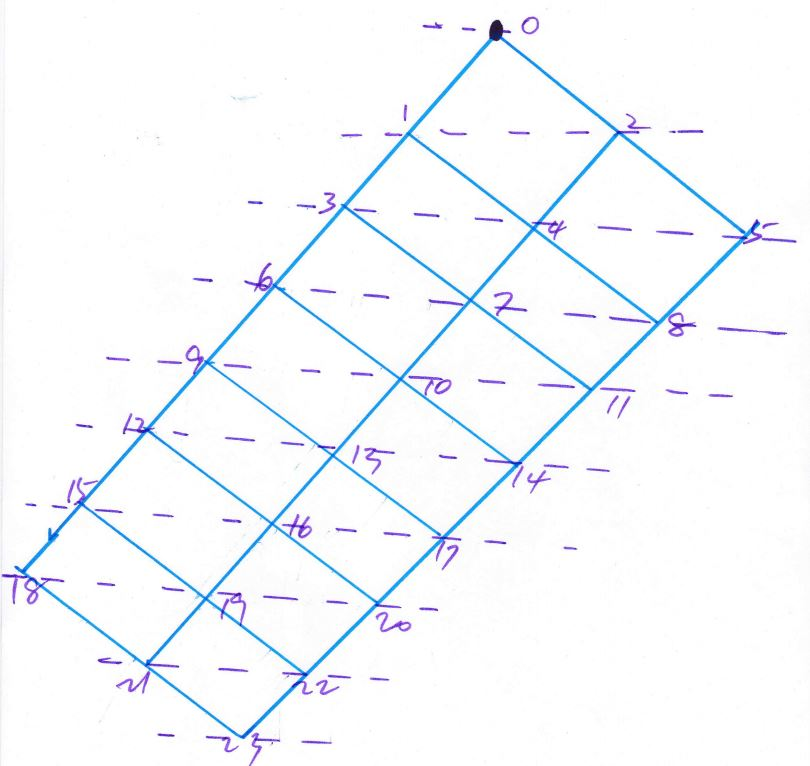
\includegraphics[width=0.55\columnwidth]{figure/3t8.JPG}
\caption{3*8 mesh network.  The data injection position is $P_{0}$}
\label{fig:3t8}
\end{figure}

Utilizing the previous methodology, we obtain the closed-form flow matrix equations for ~\ref{fig:3t8}:
\begin{equation}
{
\left[ \begin{array}{cccccccccc}
1 & 2 & 3 & 3 & 3 & 3 & 3 & 3 & 2 & 1\\
1 & -1 & 0 & 0 & 0 & 0 & 0 & 0 & 0 & 0\\
0 & \sigma-1 & 1 & 0 & 0 & 0 & 0 & 0 & 0 & 0 \\
0 & \sigma-1 & \sigma & 1 & 0 & 0 & 0 & 0 & 0 & 0 \\
0 & \sigma-1 & \sigma & \sigma & 1 & 0 & 0 & 0 & 0 & 0\\
0 & \sigma-1 & \sigma & \sigma & \sigma & 1 & 0 & 0 & 0 & 0\\
0 & \sigma-1 & \sigma & \sigma & \sigma & \sigma & 1 & 0 & 0 & 0\\
0 & \sigma-1 & \sigma & \sigma & \sigma & \sigma & \sigma & 1 & 0 & 0\\
0 & \sigma-1 & \sigma & \sigma & \sigma & \sigma & \sigma & \sigma & 1 & 0\\
0 & \sigma-1 & \sigma & \sigma & \sigma & \sigma & \sigma & \sigma & \sigma & 1 \\
\end{array} 
\right ]} \times \left[ \begin{array}{c}
\alpha_{0} \\
\alpha_{1} \\
\alpha_{3} \\
\alpha_{6} \\
\alpha_{9} \\
\alpha_{12}\\
\alpha_{15}\\
\alpha_{18}\\
\alpha_{21}\\
\alpha_{23}
\end{array} 
\right ] = \left[ \begin{array}{c}
1 \\
0 \\
0 \\
0 \\
0 \\
0 \\
0 \\
0 \\
\vdots \\
0
\end{array} 
\right ]
\end{equation}

We use the similar method to prove $\det A \neq 0$. 
The equivalence inverse processing speed :
$$T_{f,n} = 1*w_{eq}*T_{cp}$$
$$w_{eq} = \alpha_{0}*w$$

so the speedup is:
$$Speedup = \frac{T_{f, 0}}{T_{f, n}}= \frac{\omega T_{cp}}{\alpha_{0}\omega T_{cp}} = \frac{1}{\alpha_{0}} = \left |-\det A \right |$$.

The first row in flow matrix describe the number of cores on each $D_{i}$.
  For example, there is 1 core with $0$ hop distance ($D_{0}$) with load site $L$.  There are 2 cores with $1$ hop distance ($D_{1}$) with load site $L$.  There are 3 cores with $2$ hops distance ($D_{2}$) with load site $L$, and so on.
  
  The number of rows means the number of different type processor data fraction.  












